\documentclass[aspectratio=169]{beamer}
\usepackage[utf8]{inputenc}\usepackage[T1]{fontenc}\usepackage{lmodern}
\usetheme{Madrid}
\setbeamertemplate{navigation symbols}{}
\setbeamercovered{transparent}
\setbeamertemplate{itemize items}[circle]
\setbeamertemplate{enumerate items}[default]
\setlength{\parskip}{0.25em}
\definecolor{UNBCDark}{RGB}{0,74,37}
\definecolor{UNBCGold}{RGB}{189,155,96}
\definecolor{SoftGray}{RGB}{244,246,248}
\definecolor{AccentRed}{RGB}{192,57,43}
\definecolor{AccentBlue}{RGB}{41,98,255}
\definecolor{AccentTeal}{RGB}{0,150,136}
\definecolor{AccentOrange}{RGB}{230,126,34}
\setbeamercolor{normal text}{fg=black,bg=white}
\setbeamercolor{structure}{fg=UNBCDark}
\setbeamercolor{title}{fg=white,bg=UNBCDark}
\setbeamercolor{subtitle}{fg=UNBCGold}
\setbeamercolor{frametitle}{fg=white,bg=UNBCDark}
\setbeamercolor{block title}{fg=white,bg=UNBCDark}
\setbeamercolor{block body}{fg=black,bg=SoftGray}
\setbeamercolor{block title alerted}{fg=white,bg=AccentRed}
\setbeamercolor{block body alerted}{fg=black,bg=SoftGray}
\setbeamercolor{item}{fg=UNBCDark}
\setbeamercolor{alerted text}{fg=AccentRed}
\setbeamercolor{author in head/foot}{fg=white,bg=UNBCDark}
\setbeamercolor{date in head/foot}{fg=white,bg=UNBCDark}
\usepackage{booktabs,multirow,array,amsmath,amssymb,bm,graphicx,adjustbox}
\usepackage{tikz,pgfplots,multicol,tcolorbox,hyperref}
\tcbuselibrary{skins}
\pgfplotsset{compat=1.18}
\usetikzlibrary{arrows.meta,positioning,calc,decorations.pathreplacing}
\hypersetup{colorlinks=true,linkcolor=UNBCDark}
\setbeamertemplate{headline}{}
\setbeamertemplate{footline}{%
  \leavevmode\hbox{%
  \begin{beamercolorbox}[wd=.78\paperwidth,ht=2.8ex,dp=1.2ex,leftskip=1em]{author in head/foot}%
  \color{white}\textbf{ECON 308} \hspace{0.4em}\textcolor{UNBCGold}{|}\hspace{0.4em}International Economic Relations%
  \end{beamercolorbox}%
  \begin{beamercolorbox}[wd=.22\paperwidth,ht=2.8ex,dp=1.2ex,rightskip=1em plus1fil]{date in head/foot}%
  \color{white}\insertframenumber/\inserttotalframenumber%
  \end{beamercolorbox}}%
}
\newtcolorbox{insight}[1]{colback=UNBCGold!12,colframe=UNBCGold!70!black,
  title={\small\bfseries #1},left=1.5mm,right=1.5mm,top=0.8mm,bottom=0.8mm,boxrule=0.5pt,arc=2mm}
\newtcolorbox{canadex}[1][Canadian Example]{colback=AccentTeal!9,colframe=AccentTeal,
  title={\small\bfseries #1},left=1.5mm,right=1.5mm,top=0.8mm,bottom=0.8mm,boxrule=0.5pt,arc=2mm}
\newtcolorbox{discuss}{colback=AccentBlue!8,colframe=AccentBlue,
  title={\small\bfseries Discussion},left=1.5mm,right=1.5mm,top=0.8mm,bottom=0.8mm,boxrule=0.5pt,arc=2mm}
\newtcolorbox{varbox}{colback=SoftGray,colframe=UNBCDark!50,
  left=1.5mm,right=1.5mm,top=0.8mm,bottom=0.8mm,boxrule=0.4pt,arc=2mm}
\newcommand{\FIG}[1]{\begin{center}%
  \includegraphics[width=\textwidth,height=0.68\textheight,keepaspectratio]{#1}%
  \end{center}}
\newcommand{\FIGH}[2][0.85]{\begin{center}%
  \includegraphics[width=#1\textwidth,height=0.72\textheight,keepaspectratio]{#2}%
  \end{center}}

\title{\textbf{The Instruments of Trade Policy}}
\subtitle{{\large ECON 308 -- International Economic Relations \quad Chapter 9}}
\author{Muhebullah Karimzada}
\institute{School of Economics \\ University of Northern British Columbia}
\date{Fall 2026}

\begin{document}

\begin{frame}[plain]\titlepage\end{frame}

\begin{frame}{Opening Case: The Canada-US Steel Tariff Dispute (2018)}
\begin{columns}
\begin{column}{0.57\textwidth}
\begin{itemize}
  \item June 2018: US imposed 25\% tariff on Canadian steel and 10\% on aluminium under ``national security'' (Section 232).
  \item Canada retaliated with C\$12.6 billion in counter-tariffs on US goods (steel, aluminium, orange juice, ketchup, bourbon).
  \item US steel prices rose $\sim$25\%; US car and appliance manufacturers protested higher costs.
  \item The tariffs were removed in May 2019, but cost both economies real resources during the dispute.
  \item \textbf{This chapter provides the tools to analyse who paid, who gained, and how much was lost.}
\end{itemize}
\end{column}
\begin{column}{0.40\textwidth}
\FIGH[0.95]{figures/slide33_img01.PNG}
\end{column}
\end{columns}
\end{frame}

\begin{frame}{Learning Objectives}
\begin{enumerate}
  \item Distinguish specific from ad valorem tariffs and calculate their effects.
  \item Use consumer and producer surplus analysis to decompose tariff welfare effects.
  \item Derive the optimal tariff for a large country.
  \item Compare tariffs and import quotas as policy instruments.
  \item Evaluate the welfare effects of export subsidies.
  \item Apply these tools to real US/Canadian trade policy episodes.
\end{enumerate}
\end{frame}

\begin{frame}{Types of Trade Policy Instruments}
\begin{columns}
\begin{column}{0.52\textwidth}
\textbf{Tariffs:}
\begin{itemize}
  \item \textbf{Specific tariff}: fixed dollar amount per unit (e.g., \$0.25/kg of steel).
    \[P_d = P_w + t\]
  \item \textbf{Ad valorem tariff}: percentage of import value (e.g., 25\% on steel).
    \[P_d = P_w(1+\tau)\]
  \item \textbf{Tariff-rate quota (TRQ)}: low tariff up to a quota; high tariff above.
\end{itemize}
\vspace{0.3em}
\textbf{Non-tariff barriers:}
\begin{itemize}
  \item \textbf{Import quota}: physical limit on imports.
  \item \textbf{Voluntary export restraint (VER)}: foreign country ``agrees'' to limit exports.
  \item \textbf{Export subsidy}: government pays exporters per unit sold abroad.
  \item \textbf{SPS/TBT measures}: safety/standards requirements.
\end{itemize}
\end{column}
\begin{column}{0.45\textwidth}
\begin{varbox}
\small\textbf{All variables:}\\
$P_w$ = world price (exogenous for small country)\\
$P_d = P_w + t$ = domestic price after tariff\\
$t$ = specific tariff rate\\
$\tau$ = ad valorem tariff rate\\
$Q_S$ = domestic supply\\
$Q_D$ = domestic demand\\
$M = Q_D - Q_S$ = imports\\
$CS$ = consumer surplus\\
$PS$ = producer surplus\\
$GR$ = government revenue from tariff
\end{varbox}
\end{column}
\end{columns}
\end{frame}

\begin{frame}{Home Import Demand and Foreign Export Supply}
\begin{columns}
\begin{column}{0.52\textwidth}
\textbf{Deriving import demand (MD):}
\begin{itemize}
  \item At low prices: domestic demand $\gg$ supply $\Rightarrow$ large imports.
  \item As price rises: domestic supply rises and demand falls $\Rightarrow$ imports fall.
  \item MD = $Q_D(P) - Q_S(P)$: downward-sloping in price.
\end{itemize}
\vspace{0.3em}
\textbf{Foreign export supply (XS):}
\begin{itemize}
  \item At low prices: foreign industry produces little, so few exports.
  \item As price rises: foreign supply rises $\Rightarrow$ more exports.
  \item XS: upward-sloping in price.
\end{itemize}
\vspace{0.2em}
\textbf{World equilibrium}: MD $=$ XS at $P_w$.
\end{column}
\begin{column}{0.45\textwidth}
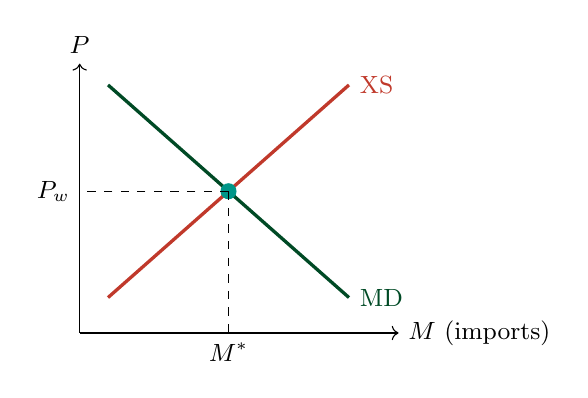
\begin{tikzpicture}[scale=0.9]
\draw[->] (0,0) -- (4.5,0) node[right]{\small $M$ (imports)};
\draw[->] (0,0) -- (0,3.8) node[above]{\small $P$};
% MD
\draw[UNBCDark,very thick] (0.4,3.5) -- (3.8,0.5) node[right]{\small MD};
% XS
\draw[AccentRed,very thick] (0.4,0.5) -- (3.8,3.5) node[right]{\small XS};
% Equilibrium
\filldraw[AccentTeal] (2.1,2.0) circle(3pt);
\draw[dashed] (2.1,2.0) -- (0,2.0) node[left]{\small $P_w$};
\draw[dashed] (2.1,2.0) -- (2.1,0) node[below]{\small $M^*$};
\end{tikzpicture}
\end{column}
\end{columns}
\end{frame}

\begin{frame}{Figure 9-5: A Tariff in a Small Country}
\begin{columns}
\begin{column}{0.54\textwidth}
\FIGH[0.96]{figures/slide16_img01.PNG}
\end{column}
\begin{column}{0.43\textwidth}
\textbf{What this figure shows:}
\begin{itemize}\small
  \item \textbf{Small country}: cannot affect world price $P_w$.
  \item A specific tariff $t$ raises the domestic price to $P_w + t$.
  \item Domestic production rises from $Q_1$ to $Q_2$ (higher price incentivises producers).
  \item Domestic consumption falls from $Q_4$ to $Q_3$ (higher price discourages consumers).
  \item Imports fall from $(Q_4-Q_1)$ to $(Q_3-Q_2)$.
  \item \textbf{Four areas}: $a$ (PS gain), $b$ (production DWL), $c$ (tariff revenue), $d$ (consumption DWL).
\end{itemize}
\end{column}
\end{columns}
\end{frame}

\begin{frame}{Consumer Surplus: The Foundation of Welfare Analysis}
\begin{columns}
\begin{column}{0.5\textwidth}
\textbf{Consumer surplus (CS)}: the difference between what consumers are \emph{willing to pay} and what they \emph{actually pay}.
\[\text{CS} = \int_0^{Q_D} D^{-1}(Q)\,dQ - P \cdot Q_D\]
Graphically: area below the demand curve and above the price.\\[0.3em]
\textbf{When price rises by $\Delta P$:}
\[\Delta\text{CS} \approx -Q_D \cdot \Delta P - \frac{1}{2}\Delta Q_D \cdot \Delta P\]
\end{column}
\begin{column}{0.47\textwidth}
\FIGH[0.96]{figures/slide22_img01.PNG}
\end{column}
\end{columns}
\end{frame}

\begin{frame}{Figure 9-6: Geometry of Consumer Surplus}
\begin{columns}
\begin{column}{0.54\textwidth}
\FIGH[0.96]{figures/slide23_img01.PNG}
\end{column}
\begin{column}{0.43\textwidth}
\textbf{Reading Figure 9-6:}
\begin{itemize}\small
  \item CS is the shaded area between the demand curve and the price line.
  \item At a \textbf{lower price}: CS is the large triangle above the low price and below the demand curve.
  \item At a \textbf{higher price}: CS shrinks to the small triangle above the high price.
  \item The \textbf{loss in CS} from a price rise = the trapezoid between the two price levels.
  \item This is exactly the area $(a+b+c+d)$ in the tariff welfare diagram.
\end{itemize}
\begin{insight}{Key message}
  Consumers always lose when prices rise from a tariff, and the loss is proportional to the price increase and the quantity affected.
\end{insight}
\end{column}
\end{columns}
\end{frame}

\begin{frame}{Figure 9-8: Geometry of Producer Surplus}
\begin{columns}
\begin{column}{0.54\textwidth}
\FIGH[0.96]{figures/slide25_img01.PNG}
\end{column}
\begin{column}{0.43\textwidth}
\textbf{Reading Figure 9-8:}
\begin{itemize}\small
  \item \textbf{Producer surplus (PS)}: area above the supply curve and below the price.
  \item PS represents \emph{profit} and rents to factors in the protected industry.
  \item When price rises from $P_w$ to $P_w + t$: PS increases by the area between the two prices and above the supply curve (area $a$).
  \item This is a \emph{transfer} from consumers to producers, not a net gain for society.
  \item But: concentrated PS gain motivates industry lobbying for protection.
\end{itemize}
\end{column}
\end{columns}
\end{frame}

\begin{frame}{Figure 9-9: Costs and Benefits of a Tariff for the Importing Country}
\begin{columns}
\begin{column}{0.54\textwidth}
\FIGH[0.96]{figures/slide27_img01.PNG}
\end{column}
\begin{column}{0.43\textwidth}
\textbf{Decomposing tariff welfare effects:}
\begin{adjustbox}{max width=\columnwidth}
\begin{tabular}{lcc}
\toprule
\textbf{Group} & \textbf{Area} & \textbf{Effect}\\
\midrule
Consumers & $-(a+b+c+d)$ & Lose\\
Producers & $+a$ & Gain\\
Government & $+c$ & Revenue\\
\midrule
\textbf{Net (small)} & $-(b+d)$ & \textbf{Lose}\\
\bottomrule
\end{tabular}
\end{adjustbox}
\vspace{0.3em}
\textbf{Area $b$}: production distortion --- resources wasted in inefficient domestic production that could have been imported more cheaply.\\[0.2em]
\textbf{Area $d$}: consumption distortion --- consumers priced out of goods they would have bought at world prices.
\end{column}
\end{columns}
\end{frame}

\begin{frame}{Figure 9-10: Net Welfare Effects of a Tariff}
\begin{columns}
\begin{column}{0.54\textwidth}
\FIGH[0.96]{figures/slide30_img01.PNG}
\end{column}
\begin{column}{0.43\textwidth}
\textbf{What Figure 9-10 shows:}
\begin{itemize}\small
  \item Consolidates the welfare analysis: net welfare change $= -(b+d)$ for a small country.
  \item \textbf{Both triangles are losses}: they represent resources misallocated due to the price distortion.
  \item The \emph{size} of the deadweight loss (DWL) depends on:
    \begin{itemize}\small
      \item The tariff rate (higher tariff $\Rightarrow$ bigger DWL).
      \item The price elasticities of supply and demand (more elastic $\Rightarrow$ bigger $b+d$).
    \end{itemize}
  \item For a \emph{large country}: there is also a ToT gain (area $e$) if world price falls. Net = $e-(b+d)$.
\end{itemize}
\end{column}
\end{columns}
\end{frame}

\begin{frame}{Figure 9-11: Average Tariffs on US Imports, 1900--2023}
\begin{columns}
\begin{column}{0.54\textwidth}
\FIGH[0.96]{figures/slide33_img01.PNG}
\end{column}
\begin{column}{0.43\textwidth}
\textbf{Historical perspective:}
\begin{itemize}\small
  \item US tariffs averaged $>$40\% in the 1930s (Smoot-Hawley, 1930).
  \item Smoot-Hawley triggered global retaliation: world trade collapsed 66\% (1929--1933).
  \item GATT rounds progressively reduced tariffs:
    \begin{itemize}\small
      \item 1947--1994: average fell from $\sim$40\% to $<$5\%.
      \item Uruguay Round (1995): WTO, $<$4\% average.
    \end{itemize}
  \item \textbf{2018 Trump tariffs}: temporary reversal --- Section 232 (steel/aluminium), Section 301 (China).
  \item Average US tariff remains $<$5\% but targeted tariffs on specific products remain high.
\end{itemize}
\end{column}
\end{columns}
\end{frame}

\begin{frame}{Figure 9-12: Annual Cost of Higher Prices by Household Income}
\begin{columns}
\begin{column}{0.54\textwidth}
\FIGH[0.96]{figures/slide35_img01.PNG}
\end{column}
\begin{column}{0.43\textwidth}
\textbf{Who bears the cost of tariffs?}
\begin{itemize}\small
  \item This figure shows the annual cost of US tariff-induced price increases by household income quintile.
  \item \textbf{Key finding}: tariffs are \emph{regressive} --- lower-income households pay a larger \emph{share} of income in higher prices.
  \item Why? Lower-income households spend more on tariffed goods (clothing, food, electronics) as a share of income.
  \item The 2018 tariffs on consumer goods from China cost US households $\sim$\$800/year on average.
  \item This regressivity is often ignored in political debates about ``protecting workers.''
\end{itemize}
\end{column}
\end{columns}
\end{frame}

\begin{frame}{The Optimal Tariff: Large-Country Case}
\begin{columns}
\begin{column}{0.52\textwidth}
\textbf{A large country} can lower the world price by restricting imports.\\[0.3em]
\textbf{Mechanism:}
\begin{enumerate}
  \item Tariff $\Rightarrow$ Home's import demand falls.
  \item Foreign export supply curve slopes up $\Rightarrow$ world price falls to $P_w'$.
  \item Home pays $P_w' + t$ domestically, but $P_w' < P_w$.
  \item Net domestic price increase $= t - (P_w - P_w') < t$.
  \item \textbf{Part of the tariff burden falls on foreign exporters}: terms of trade improve.
\end{enumerate}
\textbf{Optimal tariff formula:}
\[t^* = \frac{1}{\varepsilon_S^*}\]
where $\varepsilon_S^*$ = elasticity of foreign export supply. Lower $\varepsilon_S^*$ $\Rightarrow$ higher optimal tariff.
\end{column}
\begin{column}{0.45\textwidth}
\begin{insight}{The Optimal Tariff Temptation}
  Every large country has an incentive to impose the optimal tariff --- it improves welfare unilaterally by shifting rent from foreigners.\\[0.3em]
  But: if all countries do this simultaneously, a \emph{trade war} erupts and all are worse off. This is the \textbf{prisoner's dilemma} of trade policy --- the rationale for GATT/WTO binding commitments.
\end{insight}
\end{column}
\end{columns}
\end{frame}

\begin{frame}{Figure 9-13: Average Retaliatory Tariffs on US Exports (2018)}
\begin{columns}
\begin{column}{0.54\textwidth}
\FIGH[0.96]{figures/slide37_img01.PNG}
\end{column}
\begin{column}{0.43\textwidth}
\textbf{What this figure shows:}
\begin{itemize}\small
  \item When the US imposed tariffs in 2018, trading partners (China, EU, Canada, Mexico) retaliated with tariffs on US exports.
  \item The figure shows average retaliatory tariffs by sector.
  \item \textbf{Targeted retaliation}: foreign countries targeted sectors with political significance in the US (soy beans from Iowa, bourbon from Kentucky, motorcycles from Wisconsin --- where Harley-Davidson is headquartered).
  \item This is strategic retaliation: maximise political pressure on US politicians with minimum economic self-harm.
\end{itemize}
\end{column}
\end{columns}
\end{frame}

\begin{frame}{Import Quotas vs.\ Tariffs}
\begin{columns}
\begin{column}{0.52\textwidth}
\textbf{Import quota}: limit on physical quantity of imports.\\[0.3em]
\textbf{At equivalent restriction level}: quota raises domestic price by same amount as tariff.\\[0.3em]
\textbf{Key difference}: who captures the scarcity rent?
\begin{itemize}
  \item \textbf{Tariff}: government captures revenue (area $c$).
  \item \textbf{Quota (auctioned licences)}: equivalent to tariff.
  \item \textbf{Quota (free licences)}: rent goes to domestic importers or licence holders.
  \item \textbf{Voluntary Export Restraint (VER)}: rent accrues to \emph{foreign} exporters --- worst outcome for importing country.
\end{itemize}
\end{column}
\begin{column}{0.45\textwidth}
\begin{alertblock}{VERs: Worse than Tariffs}
  In a VER, foreign exporters \emph{voluntarily} restrict exports (under threat of worse alternatives). They capture the quota rent because their export price rises.\\[0.3em]
  The US used VERs on Japanese cars (1980s): Japanese automakers captured $\sim$\$1B/year in rents. US government got nothing.
\end{alertblock}
\vspace{0.2em}
\begin{canadex}
  Canada's dairy supply management uses TRQs: tiny quota at 0\%, then 298\% on butter above. Dairy farmers capture rents.
\end{canadex}
\end{column}
\end{columns}
\end{frame}

\begin{frame}{Figure 9-14: Effects of an Export Subsidy}
\begin{columns}
\begin{column}{0.54\textwidth}
\FIGH[0.96]{figures/slide41_img01.PNG}
\end{column}
\begin{column}{0.43\textwidth}
\textbf{What this figure shows:}
\begin{itemize}\small
  \item An export subsidy $s$ raises the price that domestic firms receive above the world price.
  \item Domestic consumers face \emph{higher} prices (less supply available domestically).
  \item World price \emph{falls} (more supply on world market).
  \item ToT \emph{deteriorate} for the exporting country.
  \item Net welfare effect:
    \begin{itemize}\small
      \item CS falls (domestic price rises).
      \item PS rises (export price rises).
      \item Government \emph{pays} the subsidy.
      \item Net: negative --- worse than a tariff.
    \end{itemize}
\end{itemize}
\begin{insight}{Export subsidies are the most costly instrument for the subsidising country.}
\end{insight}
\end{column}
\end{columns}
\end{frame}

\begin{frame}{Figure 9-15: US and World Raw Sugar Prices, 1989--2019}
\begin{columns}
\begin{column}{0.54\textwidth}
\FIGH[0.96]{figures/slide49_img01.PNG}
\end{column}
\begin{column}{0.43\textwidth}
\textbf{Reading Figure 9-15:}
\begin{itemize}\small
  \item \textbf{Blue line}: US raw sugar price (domestic, protected).
  \item \textbf{Red line}: world raw sugar price.
  \item US sugar price is consistently \emph{above} the world price --- the price wedge created by the TRQ.
  \item The premium fluctuates but has averaged $\sim$50--100\% above world price for 30+ years.
  \item \textbf{Who pays?}: US consumers of sugar and sugar-containing products (candy, soda, baked goods).
  \item \textbf{Who gains?}: US sugar cane and sugar beet producers.
\end{itemize}
\end{column}
\end{columns}
\end{frame}

\begin{frame}{Figure 9-16: Effects of the US Import Quota on Sugar}
\begin{columns}
\begin{column}{0.54\textwidth}
\FIGH[0.96]{figures/slide50_img01.PNG}
\end{column}
\begin{column}{0.43\textwidth}
\textbf{Reading Figure 9-16:}
\begin{itemize}\small
  \item The US sugar TRQ effectively functions as an import quota.
  \item \textbf{Welfare decomposition}:
    \begin{itemize}\small
      \item \textbf{CS loss}: large (US consumers pay $\approx$ 2$\times$ world price).
      \item \textbf{PS gain}: domestic sugar producers gain.
      \item \textbf{Revenue}: quota rent goes to licence holders (partly foreign exporters with TRQ access).
      \item \textbf{Net DWL}: substantial.
    \end{itemize}
  \item Estimated cost to US consumers: $>\$3$ billion/year.
  \item Estimated cost per job ``saved'' in US sugar industry: $>\$500,000$.
\end{itemize}
\end{column}
\end{columns}
\end{frame}

\begin{frame}{Summary: Effects of Alternative Trade Policies}
\begin{center}
\begin{adjustbox}{max width=0.95\textwidth,max totalheight=0.75\textheight}
\begin{tabular}{lccccc}
\toprule
\textbf{Policy} & \textbf{Dom.\ price} & \textbf{$\Delta$CS} & \textbf{$\Delta$PS} & \textbf{Gov't revenue} & \textbf{Net welfare}\\
\midrule
Tariff (small) & $P_w + t$ & $-(a+b+c+d)$ & $+a$ & $+c$ & $-(b+d)$\\
Tariff (large) & $P_w' + t$ & $-(a+b+c+d)$ & $+a$ & $+c+e$ & $e-(b+d)$\\
Import quota & $P_w + t^{\text{eq}}$ & $-(a+b+c+d)$ & $+a$ & $+c$ (if auctioned) & $-(b+d)$\\
VER & $P_w + t^{\text{eq}}$ & $-(a+b+c+d)$ & $+a$ & $0$ & $-(b+c+d)$\\
Export subsidy & $P_w + s$ & $-(a+b+c)$ & $+a+b$ & $-(b+c)$ & $-(b+c)$\\
\bottomrule
\multicolumn{6}{l}{\small Note: all compared to free trade benchmark; $e$ = ToT gain for large country.}
\end{tabular}
\end{adjustbox}
\end{center}
\vspace{0.2em}
\begin{insight}{Ranking of Instruments}
  For an importing country: Tariff $\geq$ Quota (auctioned) $>$ Quota (free) $\gg$ VER.\\
  For welfare: free trade dominates all (absent market failures or large-country effects).
\end{insight}
\end{frame}

\begin{frame}{Key Takeaways}
\begin{enumerate}
  \item Tariffs raise domestic price, protect producers, raise government revenue, and harm consumers. \textbf{Net DWL = $b + d$} for a small country.
  \item \textbf{Large countries} can gain from an optimal tariff (ToT improvement) --- but invite retaliation.
  \item \textbf{Quotas vs.\ tariffs}: similar price effects but rent allocation differs. VERs are worst (rent to foreigners).
  \item \textbf{Export subsidies} simultaneously raise domestic prices and worsen the ToT --- net welfare is negative.
  \item Real cost per job saved by protection is enormous --- far exceeds typical manufacturing wages.
  \item US 2018 tariffs cost households $\sim$\$800/year, were regressive, and invited costly retaliation.
\end{enumerate}
\begin{block}{Next: Chapter 10 --- Political Economy of Trade Policy}
  If free trade is so clearly better, why does protection persist?
\end{block}
\end{frame}

\end{document}
